\chapter{Requisiti}

\section{Requisiti funzionali}
Per la realizzare del sistema si necessita:
\begin{itemize}
	\item di un utente in possesso di uno smartphone con sistema operativo Android versione 4.3 o superiore
	\item uno o più iBeacon 
	\item un ambiente chiuso in cui disporre gli iBeacon
\end{itemize}
Nello specifico per non alterare le rilevazioni gli iBeacon devono essere disposti:
\begin{itemize}
	\item su pareti regolari a circa 1 metro da terra
	\item lontano da apparecchi che emettono onde elettromagnetiche (ad esempio router wifi) 
	\item lontano da raffiche di vento
	\item in aree in cui non si frappongano oggetti o persone tra lo smartphone e l'iBeacon target.
\end{itemize}
Per poter avere un feedback a schermo della distanza reale utente-iBeacon si necessita di:
\begin{itemize}
	\item una board Arduino UNO
	\item un sensore ultrasonico
	\item cavi di collegamento
	\item un cavo USB da stampante
	\item uno smartphone che supporti la tecnologia 
	\href{https://it.wikipedia.org/wiki/USB_On-The-Go}{\textbf{USB OTG (\textit{On-The-Go})}}\footnote{USB OTG - \url{https://it.wikipedia.org/wiki/USB_On-The-Go}}
	\item un cavo USB OTG
\end{itemize}

%\section{Requisiti non funzionali}
%???

\section{Analisi dei requisiti}
\subsection{Casi d'uso}
\begin{figure}[ph]
	\centering
	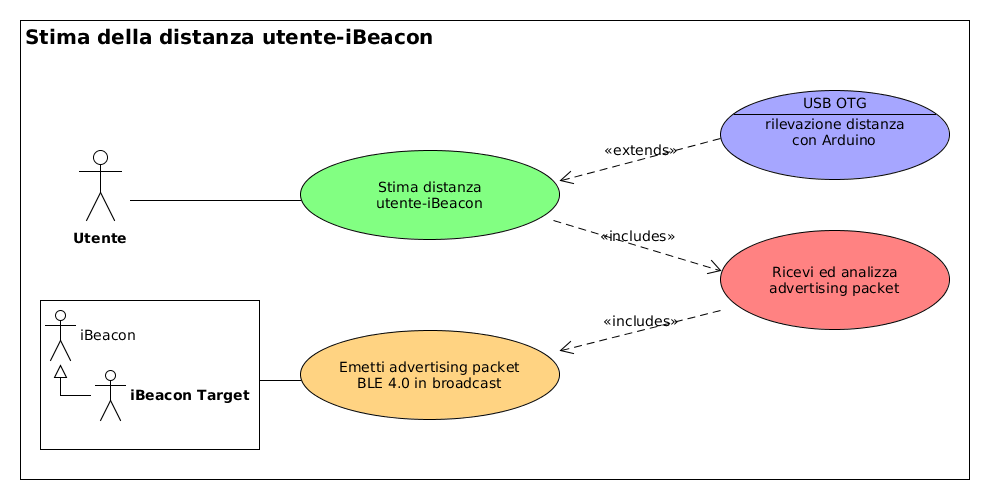
\includegraphics[scale=.45]{img/use_case/use_case1}
	\caption[Use case - Stima della distanza utente-iBeacon]{Use case - Stima della distanza utente-iBeacon}
	\label{fig:usecase}
\end{figure}

\subsection{Scenari}